\section{Neutron Diffusion Results}
\label{sec:diffusionResults}

\begin{frame}{Verification and Validation}
  \begin{itemize}
    \item ``Code Verification''
      \begin{itemize}
        \item Compare computational results to exact analytic or manufactured
          results.
        \item Demonstrate the code is solving equations correctly as designed.
        \item Quantified numerical errors.
      \end{itemize}
    \item ``Solution Verification''
      \begin{itemize}
        \item Compare computational results to benchmark results for the
          intended application of the solver.
        \item Computational results from a different method or experimental
          data.
        \item Typically verified by others previously.
      \end{itemize}
  \end{itemize}
\end{frame}

\begin{frame}{Error Analysis}
  \gls{fem} with linear elements is second-order convergent in space
  \cite{textbookli}.
  \begin{align} 
    \label{eq:error_bound}
    \ve &= \phi(\vr) - \phi_{FEM} \\
    \|\ve\|_{\infty} \le c h^2 \| \grad^2 \phi(\vr) \|_{\infty}
  \end{align}
  It is useful to define the following errors as \gls{rms} error and maximum
  error.
  \begin{align}
    \label{eq:rms}
    \text{\glsentryshort{rms}}(\ve) &= \sqrt{\frac{1}{N} \sum_{i=1}^{N} e_i^2}\\
    \label{eq:infnorm}
    \|\ve\|_{\infty} &= \max_{i=1,2,\ldots,N} \lvert e_i \rvert \\
    \label{eq:keff_err}
    \keff \; \text{ error } \units{\glsentryshort{pcm}} &= (\kref - \keff) \times 10^5
  \end{align}
  The order is second-order spatially convergent.
  \begin{equation}
    4 = \frac{e^{(i-1)}}{e^{(i)}}
  \end{equation}
\end{frame}

\begin{frame}{Analytic Solutions}
  \begin{itemize}
    \item 6 analytic multigroup neutron diffusion problems.
    \item Varied number of dimensions, energy groups, and number of materials.
  \end{itemize}
  \begin{table}
    %\caption{}
    %\label{}
    \begin{tabular}{lcccc}
      \toprule
      Case & Dimensions & Groups & Criticality & Materials \\
      \midrule
      % One-Dimension, One-Group, Fixed Source
      1 & 1 & 1 &   & 1 \\
      % One-Dimension, One-Group, Criticality
      2 & 1 & 1 & \true & 1 \\
      % Two-Dimension, One-Group, Criticality
      3 & 2 & 1 & \true & 1 \\
      % One-Dimension, Two-Group, Criticality
      4 & 1 & 2 & \true & 1 \\
      % One-Dimension, One-Group, Two-Region, Criticality
      5 & 1 & 1 & \true & 2 \\
      % Three-Dimension, One-Group, Finite Cylinder
      6 & 3 & 1 & \true & 1 \\
      \bottomrule
    \end{tabular}
  \end{table}
\end{frame}

\begin{frame}{Two-Dimension, One-Group, Criticality}
  \begin{table}
    %\caption{Two-Dimension, One-Group, Criticality Convergence Study
    %  Results.}
    \label{tab:2d1g}
    \begin{center}
      \resizebox{\textwidth}{!}{
      \begin{tabular}{cccccccccc}
        \toprule
        Refine & $\keff$ & $\keff$ error \units{\glsentryshort{pcm}} & $\keff$ ratio & 
          \gls{rms} & \gls{rms} ratio  & $\|e\|_{\infty}$ & 
          $\|e\|_{\infty}$ ratio \\
        \midrule
        \csvreader[
          late after line=\\,
          late after last line=\\,]
          {../ch03_diffusionResults/data/2d1g.csv}{}
          {\csvcoli & \csvcolii & \csvcoliii & \csvcoliv & \csvcolv & 
          \csvcolvi & \csvcolxi & \csvcolxii}
        Ref. & 1.996060  \\
        \bottomrule
      \end{tabular}
    }
    \end{center}
  \end{table}
  \begin{equation}
    \label{eq:analytic_2d1g}
    \phi(x,y) = \phi_0 \sin\left(\frac{\pi}{L_x} x\right) \, 
      \sin\left(\frac{\pi}{L_y} y\right)
  \end{equation}
\end{frame}

\begin{frame}{Two-Dimension, One-Group, Criticality}
  \begin{figure}
    \centering
    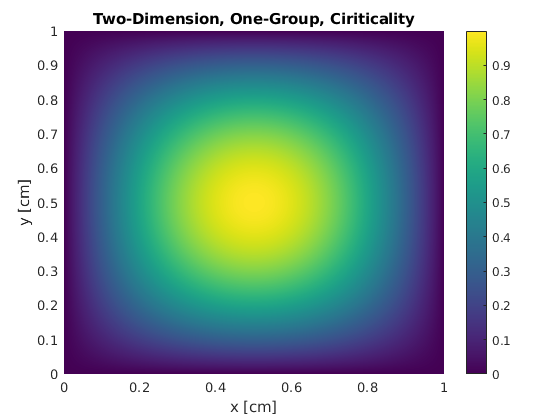
\includegraphics[width=0.7\textwidth]{2d1g}
    \caption{Two-Dimension Criticality Flux Shape.}
    \label{fig:2d1g}
  \end{figure}
\end{frame}

\begin{frame}{Three-Dimension, One-Group, Finite Cylinder}

  \begin{table}
    %\caption{Finite Cylinder Convergence Study Results.}
    \label{tab:finite_cyl}
    \begin{center}
      \resizebox{\textwidth}{!}{
      \begin{threeparttable}
      \begin{tabular}{cccccccccc}
        \toprule
        Refine & $\keff$ & $\keff$ error \units{\glsentryshort{pcm}} & $\keff$ ratio & \gls{rms} & 
          \gls{rms} ratio  & $\|e\|_{\infty}$ & $\|e\|_{\infty}$ ratio \\
        \midrule
        0     &0.895108&10160.26&4.18   &5.34E-02&2.57     &2.12E-01&1.62\\
        1     &0.972412&2429.90 &4.16   &2.07E-02&3.19     &1.31E-01&4.65\\
        2\tnote{$\dagger$}     &0.990870&584.06  &3.90   &6.50E-03&1.85     &2.81E-02&1.79\\
        3     &0.995215&149.61  &3.99   &3.51E-03&9.22     &1.57E-02&8.28\\
        4     &0.996336&37.48   &       &3.81E-04&         &1.90E-03&    \\
        Ref. & 0.996711 \\
        \bottomrule
      \end{tabular}
        \begin{tablenotes}
        \item[$\dagger$] Refinement ratio $\approx 1$ but next case $\approx
          8$.\\
          This is due to the movement of mesh nodes in the process of circular
          mesh regeneration.
        \end{tablenotes}
      \end{threeparttable}
    }
    \end{center}
  \end{table}

  \vspace{-0.2in}

  \begin{figure}
    \centering
    \subfloat{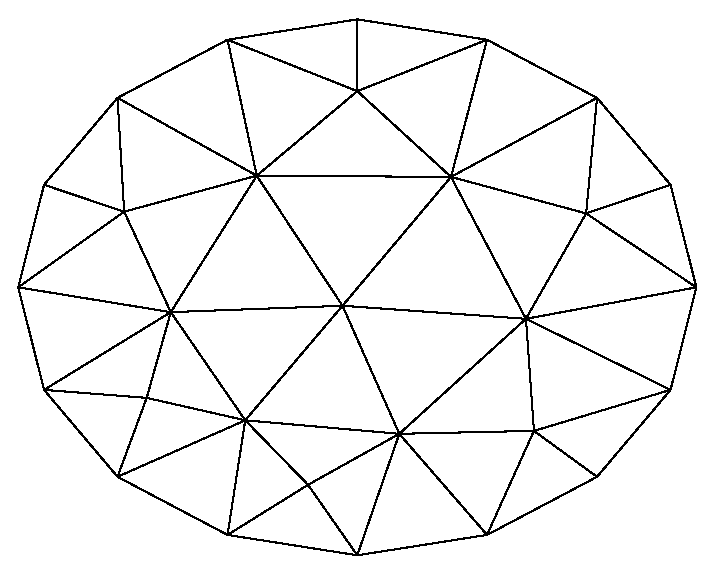
\includegraphics[width=0.35\textwidth]{cir0}}
    \vspace{0.2in}
    \subfloat{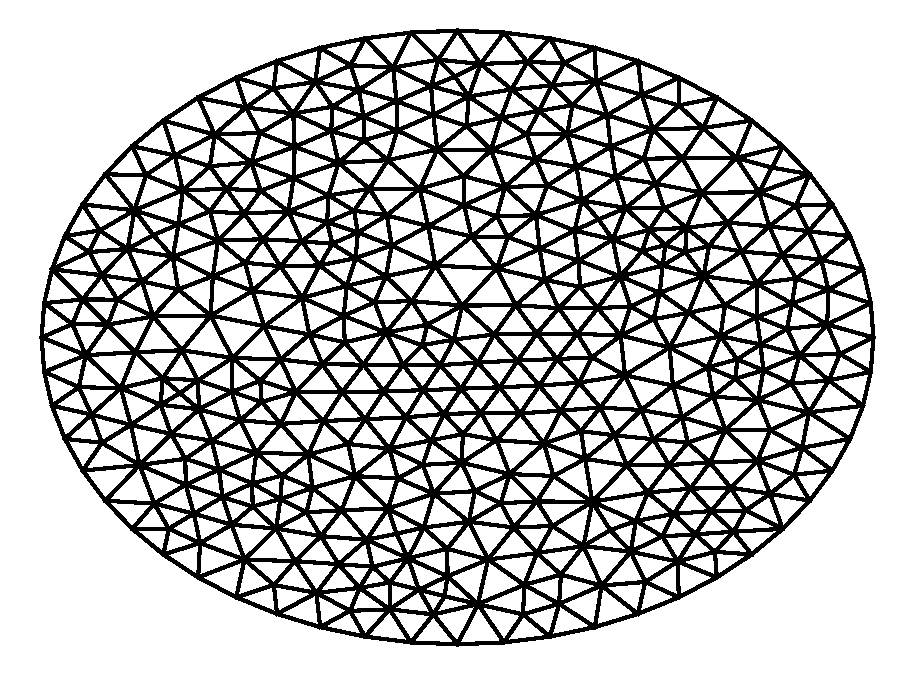
\includegraphics[width=0.35\textwidth]{cir2}}
    %\caption{Mesh Refinement of Curved Mesh.}
    \label{fig:circle_meshes}
  \end{figure}

  \vspace{-0.4in}

  \begin{equation}
    \label{eq:analytic_finite_cyl}
    \phi(r,z) = \phi_0 \, 
      J_0\left(\frac{\alpha_0}{T} r\right) \sin\left(\frac{\pi}{H} z \right)
  \end{equation}
\end{frame}

\begin{frame}{Three-Dimension, One-Group, Finite Cylinder}
  \begin{figure}
    \centering
    \subfloat{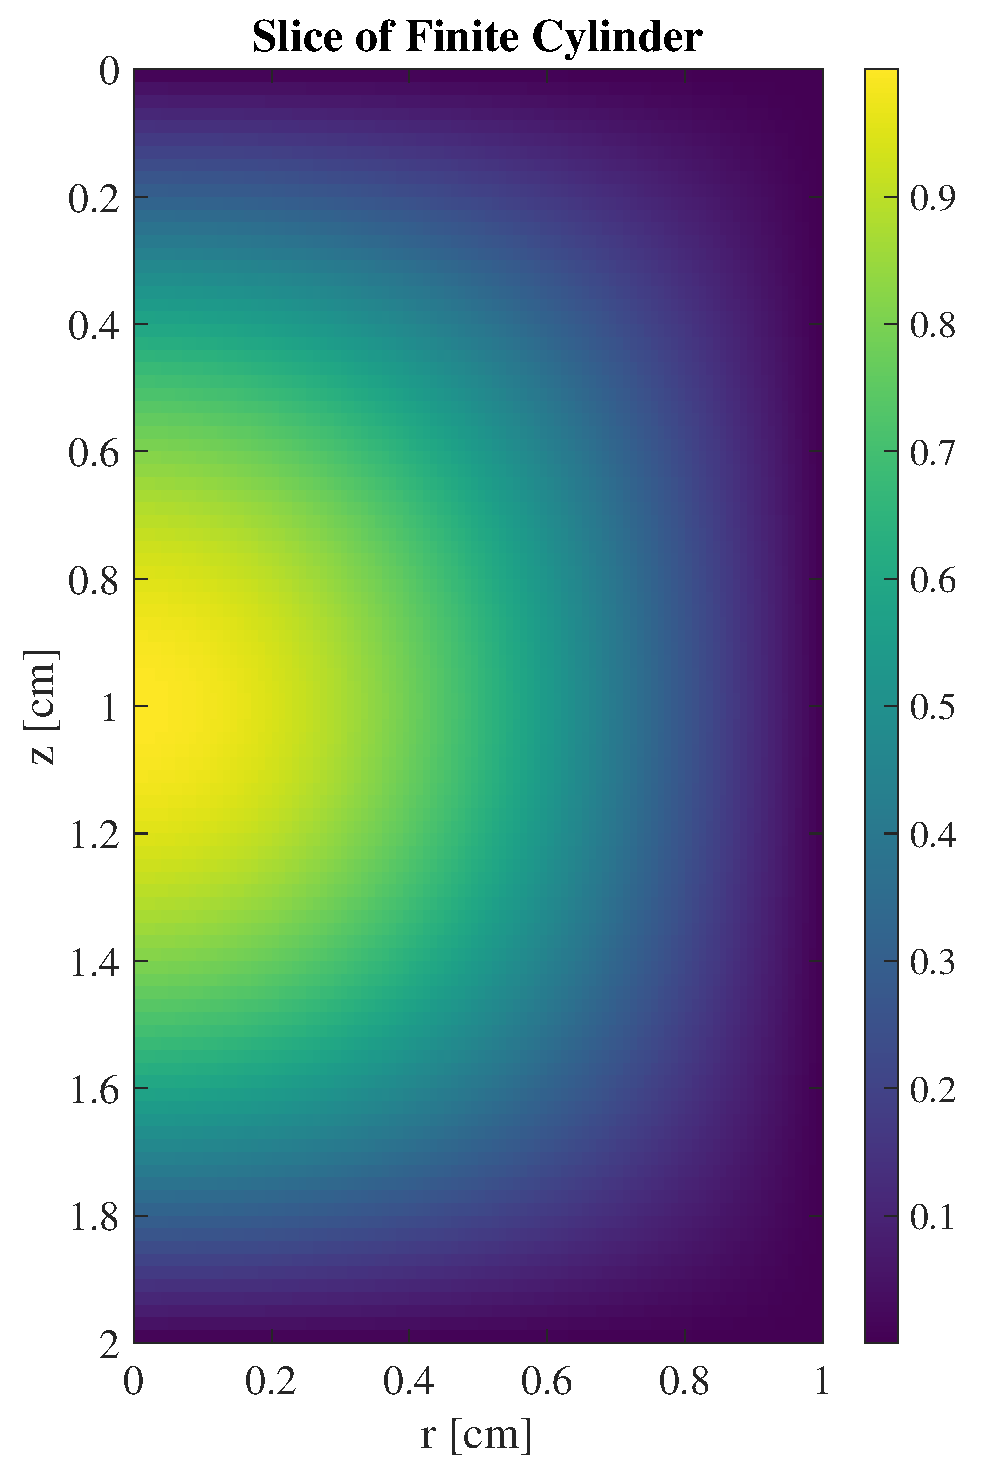
\includegraphics[width=0.4\textwidth]{finite_cyl}}
    \hspace{0.2in}
    \subfloat{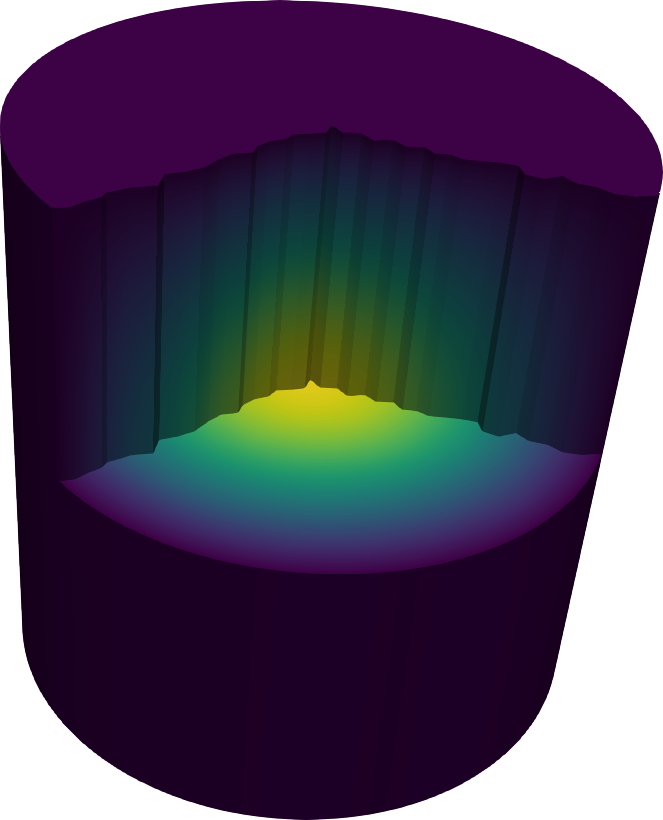
\includegraphics[width=0.4\textwidth]{./figs/finite_cyl_refine3}}
    \caption{Example Finite Cylinder Flux Shape.}
    \label{fig:finite_cyl}
  \end{figure}
\end{frame}

\begin{frame}{Benchmark Solutions}
  \begin{itemize}
    \item 9 benchmark problems.
    \item Two and three dimensions.
    \item Varied energy group structure and neutron spectrum.
  \end{itemize}
  \begin{table}
    %\caption{}
    %\label{}
    \begin{center}
      \resizebox{\textwidth}{!}{
      \begin{tabular}{lccccc}
        \toprule
        Benchmark & Dimensions & Groups & Reactor Type &
          \parbox[t]{0.6in}{\centering Neutron \\ Spectrum} \\
        \midrule
        VVER440 & 2 & 2 & \glsentryshort{lwr} & Thermal \\
        SNR     & 2 & 4 & \glsentryshort{sfr} & Fast \\
        \glsentryshort{hwr}     & 2 & 2 & \glsentryshort{hwr} & Thermal \\
        IAEA ($\times4$)    & 2 & 2 & \glsentryshort{pwr} & Thermal \\
        MONJU   & 3 & 3 & \glsentryshort{sfr} & Fast \\
        KNK     & 3 & 4 & \glsentryshort{sfr} & Fast \\
        \bottomrule
      \end{tabular}
    }
    \end{center}
  \end{table}
\end{frame}

\begin{frame}{VVER440}
  \begin{itemize}
    \item Two-dimensional.
    \item \gls{lwr}.
    \item Two-group.
  \end{itemize}
  \begin{table}
    \begin{center}
      %\caption{VVER440 Benchmark Convergence Study.}
      \label{tab:vver440}
      \begin{threeparttable}
        \begin{tabular}{cccc}
          \toprule
          Refine & $\keff$ & $\keff$ error \units{\glsentryshort{pcm}} \\
          \midrule
          \csvreader[
            late after line=\\,
            late after last line=\\,]
            {../ch03_diffusionResults/data/vver440.csv}{}
            {\csvcoli & \csvcolvi & \csvcolvii}
          Ref.\tnote{$\dagger$}  & 1.009700 \\
          \bottomrule
        \end{tabular}
        \begin{tablenotes}
          \item[$\dagger$] See \cite{chao}.
        \end{tablenotes}
      \end{threeparttable}
    \end{center}
  \end{table}
\end{frame}

\begin{frame}{VVER440 Benchmark Power Comparison}
  \begin{figure}
    \centering
    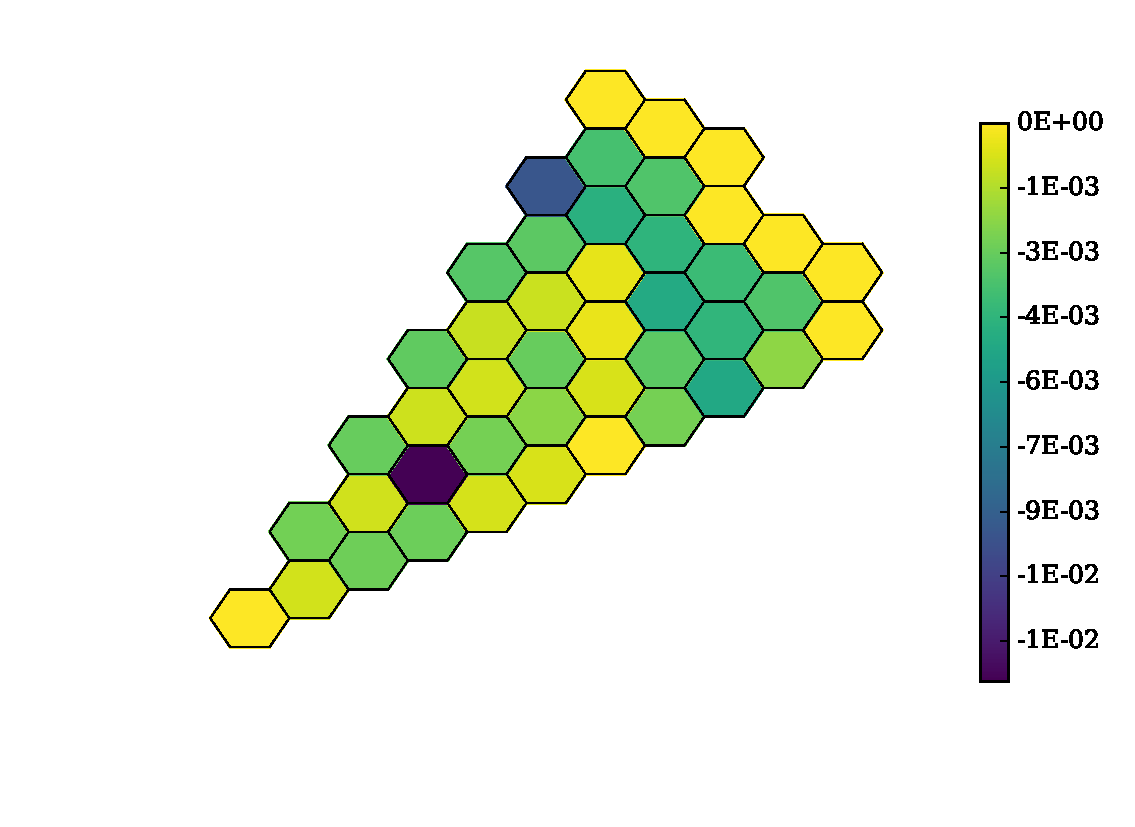
\includegraphics[width=\textwidth]{./figs/diffusion_vver440_colored}
    %\caption{VVER440 Benchmark Power Comparison for Most Refined Mesh.}
    \label{fig:diffusion_vver440}
  \end{figure}
  %\Put(25,350){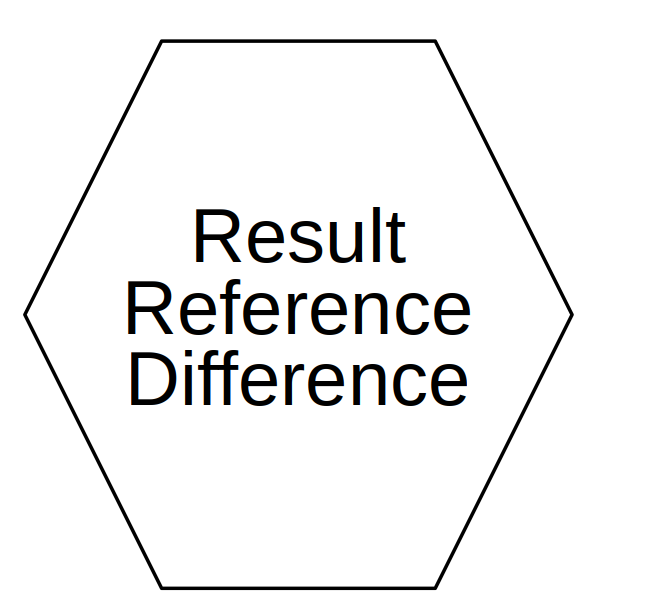
\includegraphics[width=0.15\textwidth]{hex_description}}
  \vspace{-0.5in}
  \begin{center}
    {VVER440 Benchmark Power Comparison for Most Refined Mesh.}
  \end{center}
\end{frame}

\begin{frame}{MONJU}
  \begin{itemize}
    \item Three-dimensional.
    \item \gls{sfr}.
    \item Three-group.
    \item Case A. Control rods fully removed.
    \item Case B. Control rods partially inserted.
    \item Case C. Control rods fully inserted.
    %\item Fission spectrum, $\chi$ not provided and instead selected for
    %  benchmark agreement.
  \end{itemize}
  \begin{table}
    \begin{center}
      %\caption{MONJU Benchmark Rod Worth Results. \cite{monjuBenchmark}}
      \label{tab:monju}
      \begin{threeparttable}
        \begin{tabular}{ccll}
          \toprule
          Pattern & $\keff$ & Rod Worth \units{$\Delta k$} & 
            Rod Difference \units{\%$\Delta k$} \\
          \midrule
          A&1.056816&               &            \\
          B&1.031623&0.023 (2.51E-5) \tnote{$\dagger$} &2.52 (-0.07)\\
          C&1.006519&0.047 (1.77E-3)&5.03 (0.04) \\
          \bottomrule
        \end{tabular}
        \begin{tablenotes}
          \item[$\dagger$] Value in parentheses is difference to reference
            value \cite{monjuBenchmark}.
        \end{tablenotes}
      \end{threeparttable}
    \end{center}
  \end{table}
\end{frame}
